\chapter{中等数学}
在本章中将罗列《中等数学》杂志的所有好的问题列表, 这里``好''的意思是问题表述符合竞赛难度并且问题表述无误.
当然整本杂志也存在问题本身是对的, 但解答错误的情况, 而这时将会在列出问题时给出纠正后的解答, (当然这种情况并不多见). 
由于将解答正确的回答一并抄下并不是本章的目的, 而且也没有抄的必要, 所以这里的问题基本都没有解答, 如果需要解答过程, 
则可以在本项目某个目录的角落找到当期杂志的相应问题参考解答. 另外, 由于《中等数学》杂志中一篇文章中可能会涵盖多个问题, 
所以在建立问题列表的时候做了些许偷懒, 一个问题所在的期刊和文章名字只在这篇文章中第一个被摘录的问题里给出, 而后续问题将省略详细的问题信息, 
所以在检索问题的位置时, 需要往前查找第一个遇到的带有期刊信息的问题, 然后搜索相应的杂志页.
\section{1990 年第一期}

\bq{初中数学竞赛中的逻辑推理问题}{}
某参观团根据下列约束条件, 从 $A, B, C, D, E$ 五个地方选定参观地点:
\begin{enumerate}[(1).]
	\item 若去 $A$ 地, 也必须去 $B$ 地;
	\item $D, E$ 两地至少去一地;
	\item $B, C$ 两地只去一地;
	\item $C, D$ 两地都去或都不去;
	\item 若去 $E$ 地, $A, D$ 两地也必须去.
\end{enumerate}
请你说明理由, 该参观团最多去哪几个地方?
\eq
\ba
最多去 $C,D$ 两个地方.
\ea

\bq{}{}
有甲、乙、丙、丁四位邸手参加比赛, 其中有一位歌手获奖, 有人走访了这四位歌手.

甲说:``我获了奖."

乙说:``甲没有获奖, 丙也没有获奖."

丙说:``是甲获奖或者是乙获奖."

丁说:``是乙获奖."

这四位歌手的话中, 有两句是对的. 请问: 到底是哪位歌手获奖?
\eq
\ba
甲获奖.
\ea

\bq{}{}
某刑事案件的六个嫌疑分子 $A, B, C, D, E, F$ 交待了以下材料:

$A$: $B$ 与 $F$ 做案;

$B$: $D$ 与 $A$ 做案;

$C$: $B$ 与 $E$ 做案;

$D$: $A$ 与 $C$ 做案;

$E$: $F$ 与 $A$ 做案.

司法人员根据充分的证据确信此案是两个人合作的, 且有四人各说对了一个罪犯的名字, 
一个说的全不对. 问谁是最烦?
\eq
\ba
$A$ 与 $E$.
\ea

\bq{上海市 87 年初中数学竞赛题}{}
某学校举办数学竞赛, 甲、乙、丙、丁、戊五位同学取得前五名. 发奖前, 老师让他们猜一猜各人的名次排列情况.

甲说: 乙第三名, 丙第五名;

乙说: 戊第四名, 丁第五名;

丙说: 甲第一名, 戊第四名;

丁说: 丙第一名, 乙第二名;

戊说: 甲第三名, 丁第四名.

老师说, 每个名次都有人猜对, 则获得第四名的是谁?
\eq
\ba
戊
\ea

\bq{}{}
求一个四位数, 它的 $4$ 倍恰好等于其逆序数.
\eq
\ba
$2178$.
\ea

\bq{IMO 19-2}{}
在一个实数的有限数列中, 任何 $7$ 个连续项之和都是负数, 而任何 $11$ 个连缘项之和都是正数. 试问, 这样一个数列最多能包括多少项?
\eq
\ba
$16$. 本题已被推广到任意可能的数字 $m$ 和 $n$, 结果为 $m+n-(m,n)$.
\ea

\bq{}{}
甲、乙、丙三人分别在三所大学, 学的是数学、物理、化学三个专业. 现在知道: 甲不在 $E$ 大学, 乙不在 $F$ 大学; 在 $E$ 大学的不是学物理, 在 $F$ 大学的是学数学; 乙 不是学化学. 那么, 丙上的是哪个大学? 学的什么专业?
\eq
\ba
丙在 $E$ 大学学化学.
\ea

\bq{}{}
有 $50$ 个女学生, 她们的裙子是红颜色或黄颜色, 上衣是花的或白的. 若有 $14$ 人是穿的花上衣红裙子, $31$ 人穿黄裙子, $18$ 人穿白上衣. 问穿白上衣黄裙子的有多少人?
\eq
\ba
$13$.
\ea

\bq{}{}
$A, B, C$ 三人中有两种人: 一种人只说真话, 一种人句句撒谎. $A$ 说 $B, C$ 都是撒谎的; $B$ 坚决否认; $C$ 说 $B$ 确实撒谎. 问 $A, B, C$ 中有几人说真话?
\eq
\ba
$1$ 人.
\ea

\bq{IMO 5-6}{}
五个学生 $A, B, C, D, E$ 参加一次竟赛. 有人猜测这次竟赛结果的名次是 $A B C D E$, 结果没有猜中任何一个名次, 也没有猜中任何一个学生的名次紧接在谁的后面.

另一人猜测竞赛结果的名次是 $D A E C B$, 结果猜中了两个名次, 也猜对了两个学生的名次紧接在谁后面. 问这次竞赛结果的名次是什么?
\eq
\ba
$EDACB$.
\ea

\bq{最小数原理与存在性命题, 第 26 届波兰数学竞赛}{}
已知实数列 $\left\{a_k\right\}$, ($k=1,2,3,\cdots$) 具有下列性质: 存在自然数 $n$, 满足
\bee
a_1+a_2+\cdots+a_n=0
\eee
及 $a_{n+k}=a_{k}$, ($k=1,2,3, \cdots$). 
证明: 存在自然数 $N$, 使当 $k=0,1,2, \cdots$ 时满足不等式
\bee
a_N+a_{N+1}+a_{N+2}+\cdots+a_{N+k} \ge 0.
\eee
\eq

\bq{1987 年加拿大数学竞赛}{}
在一块平地上有 $n$ 个人, 每个人到其它人的距离均不相同, 每人手中都有一把水枪, 当发出信号时, 每人用水枪击中距离他最近的人.

当 $n$ 为奇数时, 证明至少有一个人身上是干的;

当 $n$ 为偶数时, 请问这个结论是否正确?
\eq

\bq{匈牙利数学竞赛}{}
设 $P$ 是正 $n$ 边形的一个内点. 证明: 该 $n$ 边形存在两个顶点 $A$ 和 $B$. 使得
\bee
\left(1-\frac{2}{n}\right) \cdot 180^{\circ} \le \angle A P B<180^{\circ}.
\eee
\eq

\bq{1988 年加拿大数学竞赛}{}
设 $S$ 为平面上的一个有限点集 (点数 $\ge 5$), 其中若干点涂上红色, 其余的点涂上蓝色.
设任何三个或三个以上的同色的点不共线.
求证: 存在一个三角形, 使得

(1) 它的三个顶点涂有相同的颜色;

(2) 这三角形至少有一条边上不包含另一种谽色的点.
\eq

\bq{第 22 届波兰数学竞赛}{}
求最大的整数 $A$, 使对于由 $1$ 到 $100$ 的全部自然数的任一排列, 其中都有 $10$ 个位置相邻的数, 其和大于或等于 $A$.
\eq

\bq{}{}
有 $n$ 个男生, $m$ 个女生 $(n, m \ge 2)$, 每个男生至少与一女生彼此相识, 每个女生不全认识 $n$ 个男生.

证明: 他们当中必有两个男生与两个女生, 其中每个男生恰好认识其中一女生, 其中每个女生恰好认识其中一男生.
\eq

\bq{}{}
已知 $x_1, x_2, \cdots, x_n$ 是实数, $a_1, a_2, \cdots, a_n$; $b_1, b_2, \cdots, b_n$ 均是正整数. 令
\begin{align*}
	a & = \frac{a_1 x_1+a_2 x_2+\cdots+a_n x_n}{a_1+a_2+\cdots+a_n}, \\
	b & = \frac{b_1 x_1+b_2 x_2+\cdots+b_n x_n}{b_1+b_2+\cdots+b_n}.
\end{align*}
求证: 在 $x_1, x_2, \cdots, x_{n}$ 中, 必存在两数 $x_i$, $x_j$, 使下列不等式成立:
\bee
|a-b| \le \left|a-x_i\right| \le \left|x_i-x_j\right|.
\eee
\eq

\bq{}{}
平面上放了有限多个圆, 假设它们所盖住的面积为 $1$ (它们可能是彼此相交的).

试证: 一定可以从这组圆中去掉若干个圆, 使得剩下的圆互不相交, 而目它们所盖住的面积不小于 $\frac{1}{9}$.
\eq

\bq{Sylvester-Gallai 定理}{}
设 $S$ 是平面上不全共线的有限点集, 试证: 一定存在一条直线恰好通过 $S$ 中的两个点. 
\eq

\bq{}{}
在平面上给出某个点集 $M$, 使得由 $M$ 中每个点都是集 $M$ 中某两点连结线段的中点. 证明: 集合 $M$ 一定包含无穷多个点.
\eq

\bq{}{}
证明方程 $x^2+y^2=3(z^2+u^2)$ 不存在正整数解.
\eq

\bq{}{}
给定 $m n+1$ 个正整数
\bee
0<a_1<a_2<\cdots<a_{m n+1}
\eee
证明: 存在 $m+1$ 个数使它们中没有一个数能被另一数整除, 或者存在 $n+1$ 个数. 使得依大小排成序列, 除最前面的一个数之外, 每个数都能被它前面的数整除.
\eq

\bq{关于``素数无限性"的证明, Euler}{}
任意两个 Fermat 数都没有公因数
\eq

\bq{}{}
任意两个 Mersenne 数都没有公因数.
\eq

\section{根据考点划分}
\subsection{代数}
\bq{90 - 1, p. 21}{}
求 $(\sqrt{x}+2)^{2n+1}$ 的展开式中 $x$ 的整数次幂的各项系数之和.
\eq

\bq{90 - 1, p. 21}{}
设 $n\in\NN$, $A=(\sqrt{7}+2)^{2n+1}$, $B$ 为 $A$ 的小数部分, 即 $B=A-[A]$, 求证: $AB=3^{2n+1}$.
\eq

\bq{90 - 1, p. 37}{}
设 $\alpha=\alpha_1\alpha_2\cdots\alpha_N$ 是 $k$ 进制数, 
其中 $\alpha_i$, $i=1,2,\cdots, N$, $N,k$ 均为非负整数, 
且 $0\le \alpha_i\le k-1$, $k\ge 2$, $n\ge 2$. 
记 $A_{k,N}=\{\alpha|\alpha=\alpha_1\alpha_2\cdots\alpha_N\}$. 
映射 $B: A_{k,N}\to A_{k,N-1}$ 定义为: $\forall \alpha\in A_{k,N}$, 
$\beta=B(\alpha)=\beta_1\beta_2\cdots\beta_{N-1}$, 其中
$\beta_i=\min(\alpha_i,\alpha_{i+1})$, $i=1,2,\cdots,N-1$. 
记
\bee
f(k,N)=\sum_{{\alpha\in A_{k,N}}\atop{B(\alpha)=\beta}}\prod_{i=1}^{N-1}(\beta_i+1),
\eee
表示对 $A_{k,N}$ 中所有元素 $\alpha$ 关于其像 $\beta$ 的各位数字加 $1$ 
之积求和.

证明:
\begin{enumerate}
	\item $f(k,2)=\frac16k(k+1)(2k+1)$.
	\item $f(k,3)=\frac15f(k,2)(2k^2+2k+1)$.
\end{enumerate}
\eq

\subsection{三角函数}

\bq{90 - 1, p. 21}{}
化简 $\cos^2\alpha+\cos^2\beta-2\cos\alpha\cos\beta\cos(\alpha+\beta)$.
\eq

\subsection{向量}
\bq{90 - 1, p. 22}{}
对于任意的向量 $\vec{a},\vec{b},\vec{c}$, 有
\bee
(\vec{a}\times\vec{b})\times\vec{c}=(\vec{a}\cdot \vec{c}) \vec{b} - (\vec{b}\cdot\vec{c}) \vec{a}.
\eee
\eq

\subsection{复数}
\bq{90 - 1, p. 21}{}
计算:
\begin{align*}
	A & = C_n^0\cos x+C_n^1\cos 2x+\cdots+C_n^n\cos(n+1)x=\left(2\cos\frac{x}2\right)^{n}\cdot\cos\left(\frac{n+2}{2}x\right),\\
	B & = C_n^0\sin x+C_n^1\sin 2x+\cdots+C_n^n\sin(n+1)x=\left(2\cos\frac{x}2\right)^{n}\cdot\sin\left(\frac{n+2}{2}x\right).
\end{align*}
\eq

\subsection{圆锥曲线}

\bq{90 - 1, p. 31}{}
抛物线的顶点在原点, 焦点 $F$ 是圆 $x^2+y^2-4x=0$ 的圆心, 过点 $F$ 且斜率为 $2$ 的直线与抛物线交于 $A,D$, 与圆交于 $B,C$. 求 $|AB|+|CD|$.
\eq

\bq{90 - 1, p. 32}{}
$F_1,F_2$ 是椭圆的两个焦点, $P$ 是椭圆上任一点, $PF_1,PF_2$ 分别交椭圆于 $M,N$. 求证: $\frac{|PF_1|}{|F_1M|}+\frac{|PF_2|}{|F_2N|}$ 为定值.
\eq

\bq{90 - 1, p. 32}{}
设椭圆 $\frac{x^2}{a^2}+\frac{y^2}{b^2}=1$ 上两动点 $P,Q$ 在中心张直角, 即 $\angle POQ=\frac{\pi}{2}$. 试求 $\frac1{|OP|}+\frac1{|OQ|}$ 的最大值及最小值.
\eq

\subsection{几何}

\subsubsection{证明题}
\bq{90 - 1, p. 37}{}
以 $\triangle ABC$ 的三边为斜边分别向形内方向做等腰直角三角形 $BCA_1, CAB_1,ABC_1$. 
求证: $A_1, B_1, C_1$ 三点共线的充要条件是 $\cot A+\cot B+\cot C=2$.
\eq

\bq{90 - 1, p. 38}{}
平面上有两个其对应边不平行的同向相似 $n$ ($n\ge 3$) 边形 $A_1A_2\cdots A_n$ 与 $B_1B_2\cdots B_n$ (不一定是凸的). 
设 $A_i A_{i+1}$ 与 $B_i B_{i+1}$ (所在直线) 交于点 $C_i$, 过三点 $A_i, B_i, C_i$ 的圆为 $\odot O_i$ ($i=1,2,\cdots,n$, $A_{n+1}\equiv A_1$, $B_{n+1}=B_1$). 试证, 这 $n$ 个圆共点.
\eq
%\ba
%公共点是位似中心, 如图所示:
%\begin{center}
%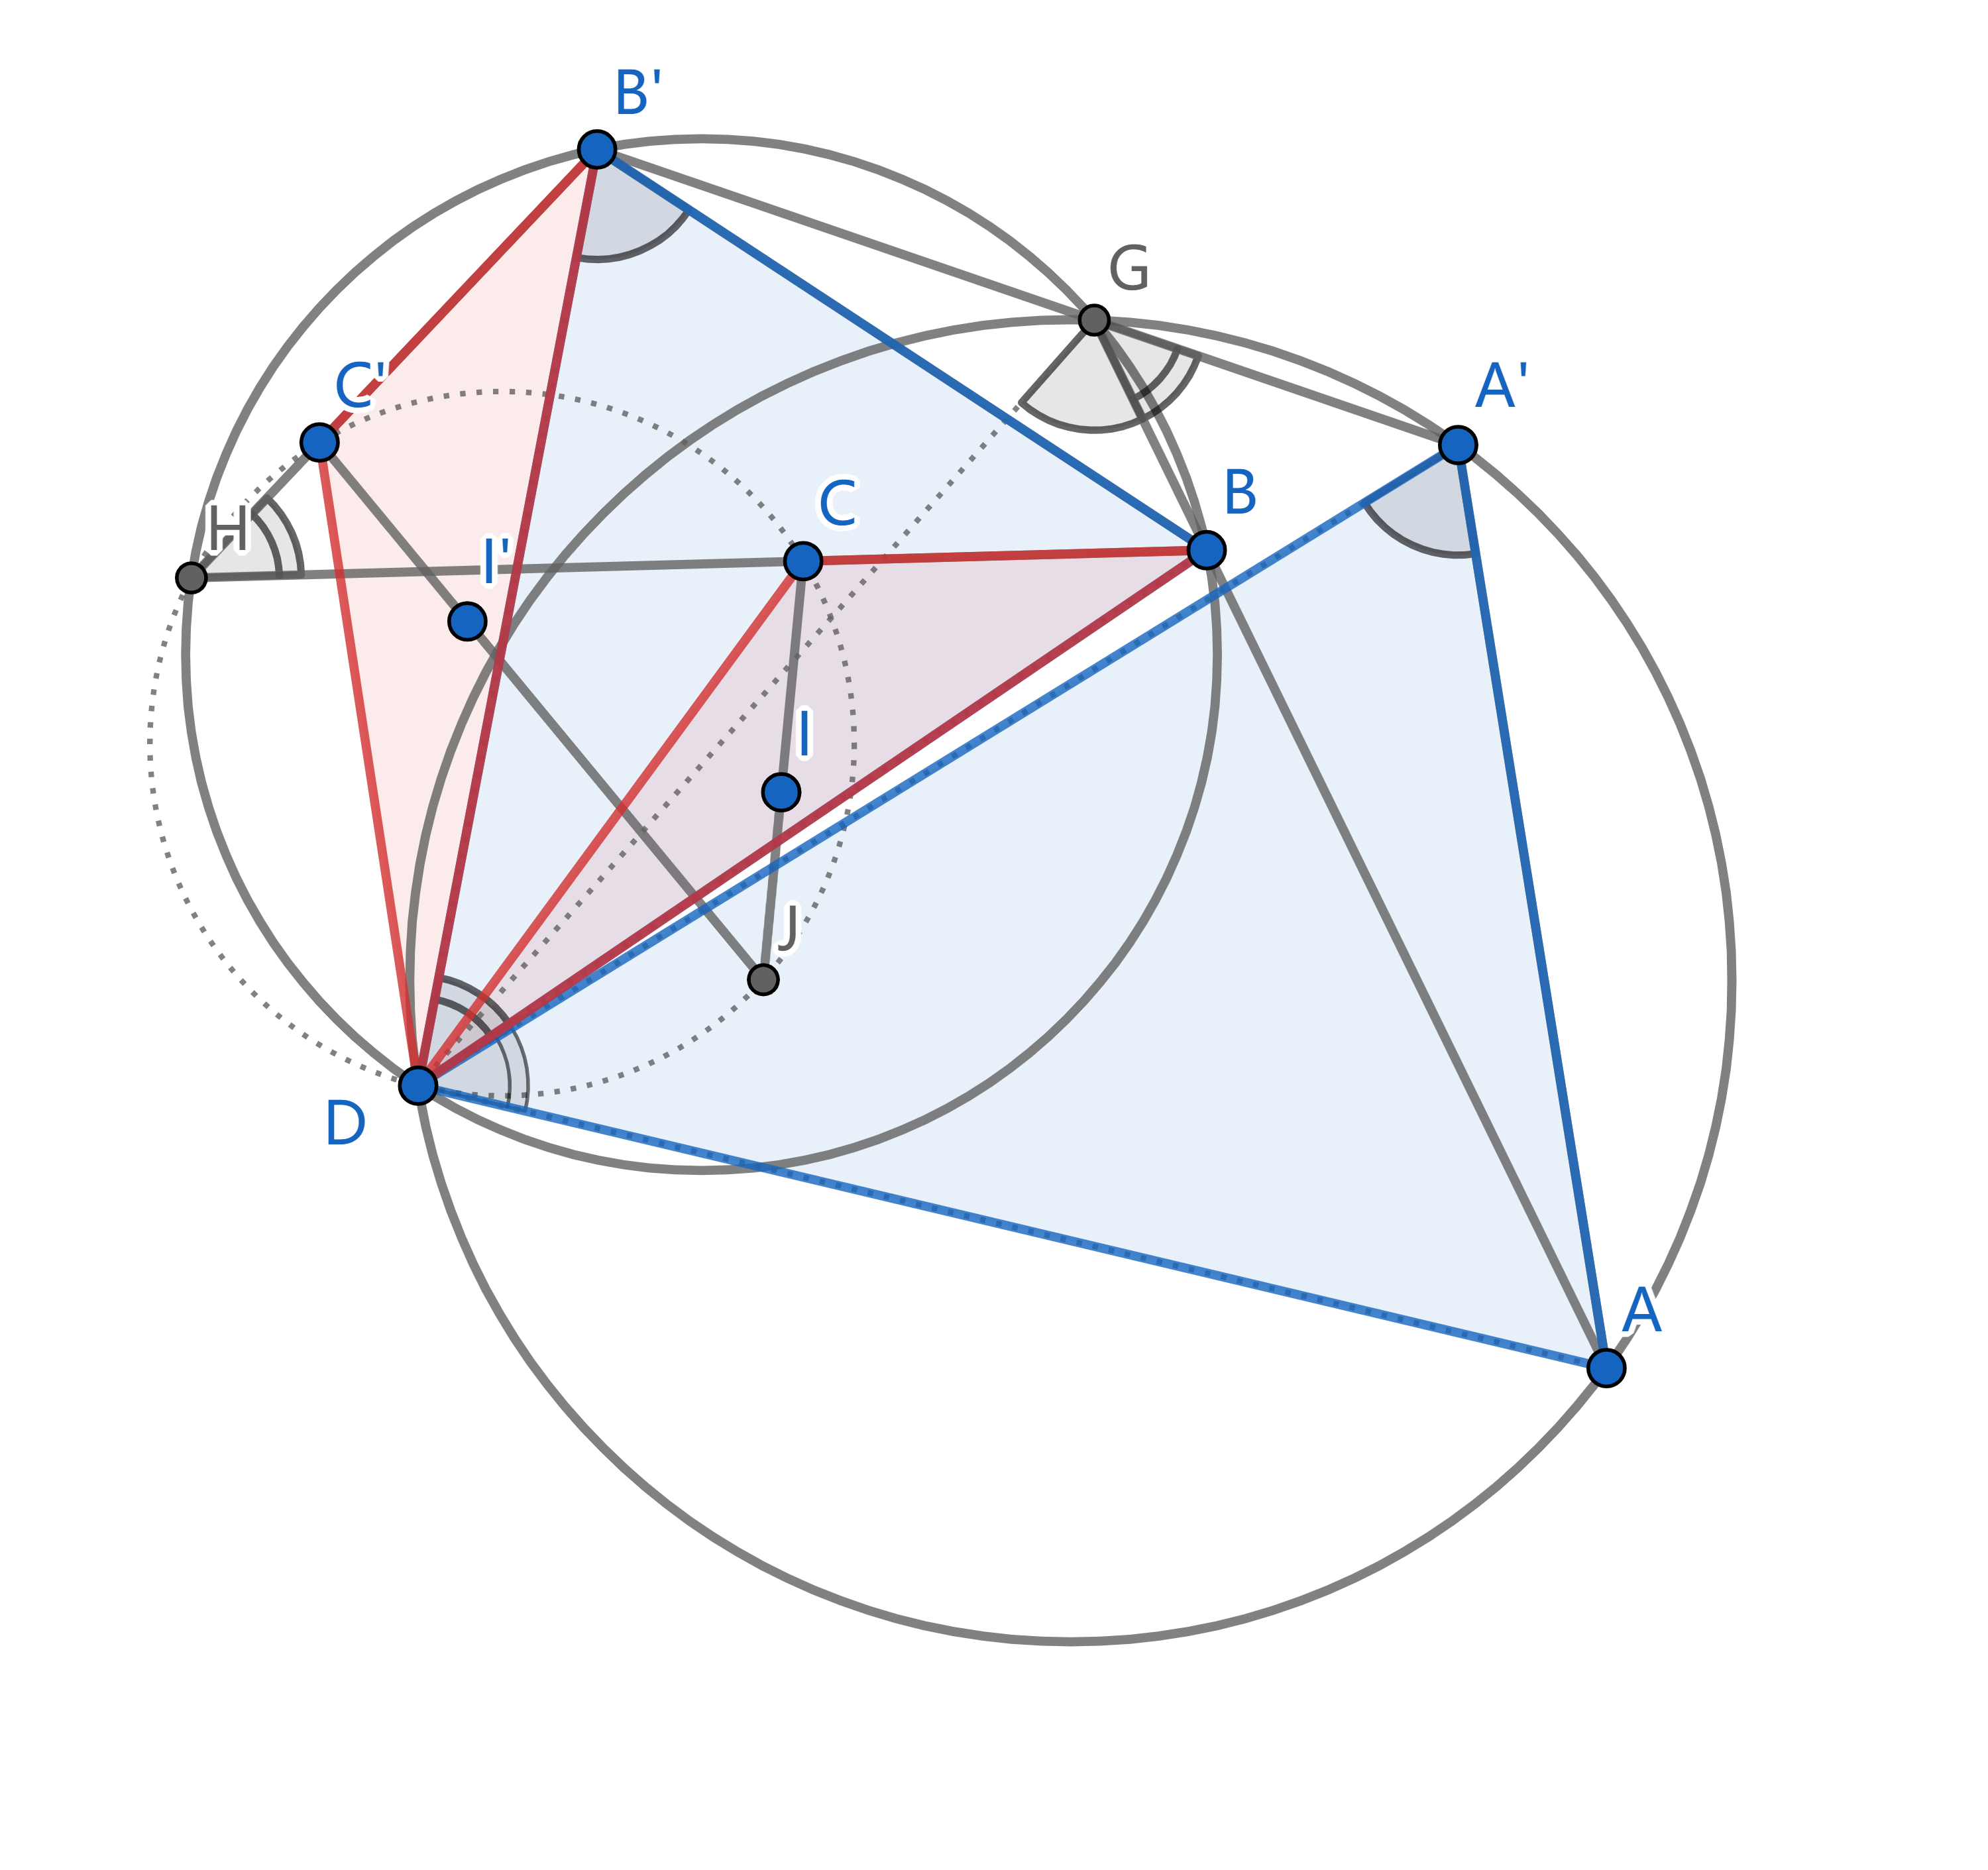
\includegraphics{imgs/2025070401.png}
%\end{center}
%\ea

\subsubsection{借助几何求解的问题}
\bq{90 - 1, p. 23}{}
已知 $x,y,z\in\RR^+$, 且满足 $x^2+xy+\frac{y^2}{3}=25$, $\frac{y^2}{3}+z^2=9$, $z^2+zx+x^2=16$, 求 $xy+2yz+3zx$ 的值.
\eq

\subsection{不等式}

\subsubsection{最值问题}
\bq{90 - 1, p. 26}{}
如果自然数 $x_1,x_2,x_3,x_4,x_5$ 满足 $x_1+x_2+x_3+x_4+x_5=x_1x_2x_3x_4x_5$, 那么 $x_5$ 的最大值是多少?
\eq

\bq{90 - 1, p. 27}{}
如果自然数 $x_1,x_2,x_3,\cdots,x_n$ 满足 $x_1+x_2+x_3+\cdots+x_n=x_1x_2x_3\cdots x_n$, 那么 $x_n$ 的最大值是多少?
\eq

\bq{90 - 1, p. 27}{}
如果自然数 $x_1,x_2,x_3,\cdots,x_n$ 满足 $x_1+x_2+x_3+\cdots+x_n=x_1x_2x_3\cdots x_n$, 那么 $x_n$ 的最大值是多少?
\eq

\subsubsection{数列不等式}
\bq{90 - 1, p. 38}{}
对每个正实数 $a_1$, 按下列方式构造数列 $a_1,a_2,\cdots$, 其中 $a_{n+1}=a_1+\frac{n}{a_n}$, ($n=1,2,\cdots$). 试求出所有使数列单调增加的 $a_1$.
\eq
%\ba
%$a_1\ge 1$.
%\ea

\subsubsection{代数不等式}
\bq{90 - 1, p. 37}{}
已知正数 $m_i$, ($i=1,2,\cdots, n$), $p\ge 2$ 且 $p$ 为正实数, 并满足
\bee
\frac1{1+m_1^p}+\frac1{1+m_2^p}+\cdots+\frac1{1+m_n^p}=1.
\eee
求证: $m_1m_2m_3\cdots m_n\ge(n-1)^{n/p}$.
\eq
\ba
设 $x_{i}=\frac{1}{1+m_{i}^{p}}$, 则有 $\sum_{i=1}^{n}x_{i}=1$. 解出
\[
m_{i}^{p}=\frac{1-x_{i}}{x_{i}}=\frac{\sum_{j\ne i}x_{j}}{x_{i}}\ge\frac{(n-1)\left(\prod_{j\ne i}x_{j}\right)^{\frac{1}{n-1}}}{x_{i}},
\]
上面的不等式为均值不等式, 所以
\[
\prod_{i=1}^{n}m_{i}^{p}\ge(n-1)^{n}.
\]
\ea

\bq{90 - 1, p. 38, 89 - 2, p. 28}{90-1}
设 $x,y,z,w\in\RR^+$, 角 $\alpha,\beta,\gamma,\theta$ 满足
\bee
\alpha+\beta+\gamma+\theta=(2k+1)\pi,\qquad k\in\ZZ.
\eee
则
\bee
x\sin\alpha+y\sin\beta+z\sin\gamma+w\sin\theta\le \sqrt{\frac{(xy+zw)(xz+yw)(xw+yz)}{xyzw}},
\eee
当且仅当 $x\cos\alpha=y\cos\beta=z\cos\gamma=w\cos\theta$ 时取等号.
\eq
%\ba
%注意到, 
%\[
%\left(x\cos\alpha-y\cos\beta\right)^{2}+\left(x\sin\alpha+y\sin\beta\right)^{2}=x^{2}+y^{2}-2xy\cos\left(\alpha+\beta\right),
%\]
%所以
%\[
%x\sin\alpha+y\sin\beta\le\sqrt{x^{2}+y^{2}-2xy\cos\left(\alpha+\beta\right)},
%\]
%等号当且仅当 $x\cos\alpha=y\cos\beta$ 时取得. 同理
%\[
%z\sin\gamma+w\sin\theta\le\sqrt{z^{2}+w^{2}-2zw\cos\left(\gamma+\theta\right)}.
%\]
%取 $a=x^{2}+y^{2}$, $b=2xy$, $c=z^{2}+w^{2}$, $d=2zw$, $\sigma=\alpha+\beta$,
%则由 $\alpha+\beta+\gamma+\theta=(2k+1)\pi$, 知
%\[
%x\sin\alpha+y\sin\beta+z\sin\gamma+w\sin\theta\le\sqrt{a-b\cos\sigma}+\sqrt{c+d\cos\sigma}.
%\]
%由加权均值不等式
%\[
%\frac{\lambda\sqrt{a}+\mu\sqrt{b}}{\lambda+\mu}\le\sqrt{\frac{\lambda a+\mu b}{\lambda+\mu}},
%\]
%\begin{align*}
%	\sqrt{a-b\cos\sigma}+\sqrt{c+d\cos\sigma} & =\frac{\lambda\cdot\frac{1}{\lambda}\sqrt{a-b\cos\sigma}+\mu\cdot\frac{1}{\mu}\sqrt{c+d\cos\sigma}}{\lambda+\mu}\cdot\left(\lambda+\mu\right)\\
%	& \le\sqrt{\frac{\lambda\cdot\frac{a-b\cos\sigma}{\lambda^{2}}+\mu\cdot\frac{c+d\cos\sigma}{\mu^{2}}}{\lambda+\mu}}\cdot\left(\lambda+\mu\right)\\
%	& =\sqrt{\left(\lambda+\mu\right)\left(\frac{a}{\lambda}+\frac{c}{\mu}+\left(\frac{d}{\mu}-\frac{b}{\lambda}\right)\cos\sigma\right)}\\
%	& =\sqrt{\frac{(ad+bc)(b+d)}{bd}},
%\end{align*}
%其中最后一步令 $\frac{d}{\mu}=\frac{b}{\lambda}$ 以消去变动项 $\cos\sigma$, 等式当且仅当
%$\frac{\sqrt{a-b\cos\sigma}}{\lambda}=\frac{\sqrt{c+d\cos\sigma}}{\mu}$
%取得, 也即 $\frac{x\sin\alpha+y\sin\beta}{2xy}=\frac{z\sin\gamma+w\sin\theta}{2zw}$,
%解得 $x\cos\alpha=z\cos\gamma$. 回带便有
%\[
%x\sin\alpha+y\sin\beta+z\sin\gamma+w\sin\theta\le\sqrt{\frac{\left(xy+zw\right)\left(xz+yw\right)\left(xw+yz\right)}{xyzw}}.
%\]
%\ea

\subsubsection{几何不等式}
\bq{88 - 1, p. 23}{}
设 $\alpha+\beta+\gamma=\pi$, 则有
\bee
\sin\alpha+\sin\beta+\sin\gamma\le \frac{3\sqrt{3}}{2},
\eee
当且仅当 $\alpha=\beta=\gamma$ 时等号成立.
\eq
%\ba
%其推广形式见问题 \ref{q:90-1}, 取 $\theta=0$, $w=\frac12$ 即可. 或参考推广形式: 问题 \ref{q:2025070603}.
%\ea

\bq{88 - 1, p. 23, Vasic}{}
设 $\alpha+\beta+\gamma=\pi$, $x,y,z\in\RR^+$, 则有
\bee
x\sin\alpha+y\sin\beta+z\sin\gamma\le \frac{\sqrt{3}}{2}\left(\frac{yz}{x}+\frac{zx}{y}+\frac{xy}{z}\right),
\eee
当且仅当 $x=y=z$, 且 $\alpha=\beta=\gamma$ 时取等号.
\eq
%\ba
%其推广形式见问题 \ref{q:90-1}, \ref{q:2025070603}, 记 $\theta=0$, 则 $\forall w>0$, 有
%\bee
%x\sin\alpha+y\sin\beta+z\sin\gamma\le\sqrt{\frac{(xy+zw)(yz+xw)(zx+yw)}{xyzw}},
%\eee
%取 $a=\frac{yz}{x}$, $b=\frac{zx}{y}$, $c=\frac{xy}{z}$, 令 $\sigma_1=a+b+c$, $\sigma_2=ab+bc+ca$, $\sigma_3=abc$. 则有
%\begin{align*}
%x\sin\alpha+y\sin\beta+z\sin\gamma
%	& \le\min_{w>0}\sqrt{\frac{(w+a)(w+b)(w+c)}{w}}\\
%	& =\min_{w>0}\sqrt{\frac{w^3+\sigma_1 w^2+\sigma_2 w+\sigma_3}{w}}\\
%	& \le\min_{w>0}\sqrt{\frac{w^3+\sigma_1 w^2+\frac{\sigma_1^2}{3} w+\frac{\sigma_1^3}{27}}{w}}\\
%	& \xlongequal{w=\sigma_1/6}\sqrt{\frac34\sigma_1^2}.
%\end{align*}
%\ea

\bq{88 - 1, p. 23, Klamkin}{}
设 $\alpha+\beta+\gamma=\pi$, $x,y,z\in\RR^+$, 则有
\bee
x\sin\alpha+y\sin\beta+z\sin\gamma\le \frac{yz+zx+zy}2\sqrt{\frac{x+y+z}{xyz}},
\eee
当且仅当 $x=y=z$, 且 $\alpha=\beta=\gamma$ 时取等号.
\eq
%\ba
%在问题 \ref{q:2025070603} 中取 $\lambda=x$, $\mu=y$, $\nu=z$.
%\ea

\bq{\cite{ZYC}, p. 48}{zyc0706}
如果 $x,y,z\in\RR$, $A+B+C=\pi$, 则
\bee
x^2+y^2+z^2\ge 2yz\cos A+2zx\cos B+2xy\cos C,
\eee
当且仅当
\bee
\begin{cases}
	x=y\cos C+z\cos B,\\
	y\sin C=z\sin B
\end{cases}
\eee
时取等号.
\eq

\bq{88 - 1, p. 23}{2025070601}
设 $x_{1},x_{2},x_{3}$ 是任意实数, $\alpha_{1},\alpha_{2},\alpha_{3}$
是任意实数, 且 $\alpha_{1}+\alpha_{2}+\alpha_{3}=(2k+1)\pi$, ($k\in\ZZ$),
则有
\[
\sum_{cyc}x_{2}x_{3}\cos\alpha_{1}\le\frac{1}{2}\sum_{cyc}x_{1}^{2},
\]
当且仅当 $x_{2}x_{3}\sin\alpha_{1}=x_{3}x_{1}\sin\alpha_{2}=x_{1}x_{2}\sin\alpha_{3}$
时取等号.
\eq
%\ba
%参考问题 \ref{q:zyc0706}.
%\ea

\bq{88 - 1, p. 23}{2025070602}
若 $\theta_{1},\theta_{2},\theta_{3}\in\RR^{+}$, $\alpha_{1},\alpha_{2},\alpha_{3}$
是任意实数, 且 $\alpha_{1}+\alpha_{2}+\alpha_{3}=(2k+1)\pi$, ($k\in\ZZ$), $\theta_{1}+\theta_{2}+\theta_{3}=\pi$,
则
\[
\sum_{cyc}\frac{x_{2}x_{3}\cos\alpha_{1}}{\sin\theta_{1}}\le\sum_{cyc}\frac{x_{2}^{2}+x_{3}^{2}}{2}\cot\theta_{1},
\]
当且仅当 $\frac{x_{2}x_{3}\sin\alpha_{1}}{\sin\theta_{1}}=\frac{x_{3}x_{1}\sin\alpha_{2}}{\sin\theta_{2}}=\frac{x_{1}x_{2}\sin\alpha_{3}}{\sin\theta_{3}}$
时取等号. 
\eq
%\ba
%注意到 $\frac1{\sin\theta_1}=\sqrt{\cot\theta_3+\cot\theta_1}\cdot\sqrt{\cot\theta_1+\cot\theta_2}$,
%并使用问题 \ref{q:2025070601}.
%\ea

\bq{88 - 1, p. 23}{2025070603}
设 $x,y,z$ 是使 $xyz>0$ 的任意实数, $\lambda,\mu,\nu\in\RR^{+}$, 且 $\alpha+\beta+\gamma=n\pi$,
($n\in\ZZ$), 则有
\[
\sum_{cyc}x\sin\alpha\le\frac{1}{2}\sqrt{\frac{\lambda+\mu+\nu}{\lambda\mu\nu}}\sum_{cyc}\frac{\lambda yz}{x},
\]
当且仅当
\[
\begin{cases}
	\frac{x}{\lambda}\sin\alpha=\frac{y}{\mu}\sin\beta=\frac{z}{\nu}\sin\gamma,\\
	x\cos\alpha=y\cos\beta=z\cos\gamma
\end{cases}
\]
时取等号.
\eq

\bq{88 - 1, p. 23}{}
对于任意的 $\alpha,\beta,\gamma\in\RR$ 满足 $\alpha+\beta+\gamma=n\pi$,
$n\in\ZZ$, 则对于任意的 $\lambda,\mu,\nu\in\RR^{+}$ 有不等式
\[
\left|\sin2\alpha+\sin2\beta+\sin2\gamma\right|\le2\left(\lambda\cos^{2}\alpha+\mu\cos^{2}\beta+\nu\cos^{2}\gamma\right)\cdot\sqrt{\frac{\lambda+\mu+\nu}{\lambda\mu\nu}},
\]
当且仅当 $\frac{\tan\alpha}{\lambda}=\frac{\tan\beta}{\mu}=\frac{\tan\gamma}{\nu}$
时取等号.
\eq
%\ba
%在问题 \ref{q:2025070603} 中令 $x=\cos\beta\cos\gamma$ 等, 如果等式左边出现负值, 用 $-\alpha$ 代 $\alpha$
%等等即可.
%\ea

\bq{88 - 1, p. 23}{}
设 $\lambda,\mu,\nu\in\RR^{+}$, $\alpha,\beta,\gamma\in(0,\pi)$,
且 $\alpha+\beta+\gamma=\pi$, 则有 
\[
\sqrt{\lambda\mu\nu(\lambda+\mu+\nu)}\le\sum_{cyc}\frac{\lambda(\mu+\nu)}{2}\cot\alpha,
\]
当且仅当 $\lambda\cot\alpha=\mu\cot\beta=\nu\cot\gamma$ 时取等号.
\eq

\bq{88 - 1, p. 23}{}
设 $\lambda,\mu,\nu\in\RR^{+}$, $\alpha,\beta,\gamma\in(0,\pi)$,
且 $\alpha+\beta+\gamma=\pi$, 则有 
\[
\sum_{cyc}\frac{\lambda+\mu}{2}\cot\gamma\ge\sqrt{\sum\limits_{cyc}\lambda\mu},
\]
当且仅当 $\lambda\tan\alpha=\mu\tan\beta=\nu\tan\gamma$ 时取等号.
\eq

\bq{88 - 1, p. 23}{}
设 $a,b,c$ 是三角形三边长, $S$ 为其面积, $\alpha,\beta,\gamma\in(0,\pi)$, 且
$\alpha+\beta+\gamma=\pi$, 则有
\[
\sum_{cyc}a\cot\alpha\ge\sqrt{4\sqrt{3}S},
\]
当且仅当 $a=b=c$, 且 $\alpha=\beta=\gamma=\frac{\pi}{3}$ 时取等号.
\eq

\bq{88 - 1, p. 23}{}
设 $a,b,c$ 是三角形三边长, $S$ 为其面积, $\lambda,\mu,\nu\in\RR^{+}$, 则有
\[
\left(\sum_{cyc}\lambda a\right)^{2}\ge4\sqrt{3}S\left(\sum_{cyc}\lambda\mu\right),
\]
当且仅当 $a=b=c$, 且 $\lambda=\mu=\nu$ 时取等号.
\eq

\bq{88 - 1, p. 23}{}
设三角形 $ABC$ 及 $A'B'C'$ 的边长分别为 $a,b,c$ 及 $a',b',c'$, 面积分别为 $S,S'$,
则有
\[
\sum_{cyc}a'(-a+b+c)\ge\sqrt{24SS'},
\]
当且仅当 $\triangle ABC$ 及 $\triangle A'B'C'$ 均是正三角形时取等号.
\eq

\bq{88 - 1, p. 23}{2025070604}
设 $a,b,c$ 及 $S$ 分别表示三角形三边长及面积, $\lambda,\mu,\nu\in\RR^{+}$, 则有
\[
\sum_{cyc}\lambda a^{2}\ge4S\sqrt{\sum_{cyc}\lambda\mu},
\]
当且仅当 $\frac{a^{2}}{\mu+\nu}=\frac{b^{2}}{\lambda+\nu}=\frac{c^{2}}{\lambda+\mu}$
时取等号.
\eq
%\ba
%只需在问题 \ref{q:2025070603} 中令 $x=\frac{bc}{\mu\nu}$ 等, 并令 $\lambda\to\frac{1}{\lambda}$
%即可.
%\ea

\bq{88 - 1, p. 23}{}
设点 $P$ 是 $\triangle ABC$ 内任意一点, $\lambda,\mu,\nu\in\RR^{+}$, 则
\[
\sum_{cyc}\lambda \cdot PA^{2}\ge\sqrt{\frac{\lambda\mu\nu}{\lambda+\mu+\nu}}\cdot4S,
\]
其中 $S$ 为 $\triangle ABC$ 的面积, 等号当且仅当 
\[
\begin{cases}
	\frac{\cos\angle BPC}{PA}=\frac{\cos\angle CPA}{PB}=\frac{\cos\angle APB}{PC},\\
	\lambda\cot\angle BPC=\mu\cot\angle CPA=\nu\cot\angle APB
\end{cases}
\]
时取到.
\eq
%\ba
%在问题 \ref{q:2025070603} 中令 $x=PB\cdot PC$ 等, $\alpha=\angle BPC$ 等即可.
%\ea

\bq{88 - 1, p. 23, Daniel Pedoe 不等式}{}
设三角形 $ABC$ 与 $A'B'C'$ 的三条边分别为 $a,b,c$ 与 $a',b',c'$, 面积分别为 $S,S'$,
则有
\[
\sum_{cyc}a'{}^{2}\left(-a^{2}+b^{2}+c^{2}\right)\ge16SS',
\]
当且仅当 $\triangle ABC\sim\triangle A'B'C'$ 时取等号.
\eq
%\ba
%令 $\lambda=-a'^2+b'^2+c'^2$ 等, 然后用问题 \ref{q:2025070604}, 并应用恒等式:
%\bee
%\sum_{cyc}(a^2+b^2-c^2)(b^2+c^2-a^2)=16S^2.
%\eee
%\ea

\bq{90 - 1, p. 21, Weitjenbok 不等式}{}
设 $\triangle ABC$ 的边和面积分别为 $a,b,c$ 和 $\triangle$, 则 $a^2+b^2+c^2\ge 4\sqrt{3}\triangle$.
\eq

\bq{88 - 1, p. 23, TODO}{}
设 $\triangle ABC$ 内任意一点 $P$ 向各边或其延长线作垂线, 设 $\triangle ABC$ 和所得垂足三角形的面积分别为 $S,S'$, 则有 $S\ge 4S'$, 
当且仅当 $P$ 是 $\triangle ABC$ 的外心时取等号.
\eq

\bq{90 - 1, p. 28, 88 年全国高中数学竞赛}{}
如图, $P,Q,R$ 将 $\triangle ABC$ 的周长三等分, 且 $P,Q\in AB$. 求证 $S_{\triangle PQR}>\frac29S_{\triangle ABC}$.
\begin{center}
	\begin{tikzpicture}[scale=1.5]
		% Define the main triangle
		\coordinate (A) at (1,3);
		\coordinate (B) at (-2,0);
		\coordinate (C) at (2,0);
		
		% Define additional points inside the triangle
		\coordinate (P) at ($(A)!1/3!(B)$);
		\coordinate (Q) at ($(B)!1/3!(C)$);
		\coordinate (R) at ($(C)!1/3!(A)$);
		
		% Draw the main triangle
		\draw (A) -- (B) -- (C) -- cycle;
		
		% Draw the additional lines
		\draw[red] (P) -- (Q) -- (R) -- cycle;
		
		% Label the points
		\node[above] at (A) {$A$};
		\node[below] at (B) {$B$};
		\node[below] at (C) {$C$};
		\node[left] at (P) {$P$};
		\node[below] at (Q) {$Q$};
		\node[right] at (R) {$R$};
	\end{tikzpicture}
\end{center}
\eq

\bq{90 - 1, p. 28, 84 年全国高中数学竞赛}{}
如图, $P\in BC$, $PE\parallel AB$ 交 $AC$ 于 $E$, $PF\parallel AC$ 交 $AB$ 于 $F$, 设 $S_{\triangle ABC}=1$. 
求证: $S_{\triangle BPF}, S_{\triangle CPE}, S_{AEPF}$ 中至少有一个不小于 $\frac49$.
\begin{center}
	\begin{tikzpicture}[scale=1.5]
		% Define the main triangle
		\coordinate (A) at (0,2);
		\coordinate (B) at (-2,0);
		\coordinate (C) at (2,0);
		
		% Define point P between P5 and P6
		\coordinate (P) at ($(B)!2/5!(C)$);
		
		% Define points F, E, D, M, H, N
		\coordinate (F) at ($(B)!(P)!(A)$); % Intersection of PF and AB
		\coordinate (E) at ($(C)!(P)!(A)$); % Intersection of PE and AC
		
		% Draw the main triangle
		\draw (A) -- (B) -- (C) -- cycle;
		
		% Draw the additional lines
		\draw (P) -- (F);
		\draw (P) -- (E);
		
		% Label the points
		\node[above] at (A) {$A$};
		\node[below] at (B) {$B$};
		\node[below] at (C) {$C$};
		\node[below] at (P) {$P$};
		\node[left] at (F) {$F$};
		\node[right] at (E) {$E$};
	\end{tikzpicture}
\end{center}
\eq

\bq{90 - 1, p. 38, 本题有误已在知乎提问}{}
如图, $AD$ 为 $BC$ 上高线, $BE$ 为 $AC$ 上中线, $CF$ 为 $\angle C$ 平分线. 三线两两交于$P$, $Q$, $R$. 
$D$ 在 $BC$ 上, 且可重于 $B$ 或 $C$. 令 $x=\frac{S_{\triangle PQR}}{S_{\triangle ABC}}$. 
求证: $x<\frac16$, 且 $x$ 可以无线接近 $\frac16$.
\eq

\bq{90 - 1, p. 28, 第 3 届 IMO}{}
$P$ 为 $\triangle ABC$ 内任一点, $AP,BP,CP$ 分别交对边于 $P_1,P_2,P_3$. 求证: $\frac{AP}{PP_1},\frac{BP}{PP_2},\frac{CP}{PP_3}$ 中至少有一个不大于 $2$, 也至少有一个不小于 $2$.
\eq

\bq{90 - 1, p. 28, 78 年安徽省数学竞赛}{}
过三角形重心的任一直线把这三角形分成两部分, 求证这两部分面积之差不大于整个三角形的 $\frac19$.
\eq

\bq{90 - 1, p. 23}{}
已知 $\alpha,\beta,\gamma$ 为锐角, 且 $\cos^2\alpha+\cos^2\beta+\cos^2\gamma=1$, 求证: $\tan\alpha\tan\beta\tan\gamma\ge 2\sqrt{2}$.
\eq

\subsubsection{立体几何不等式}
\bq{90 - 1, p. 38}{}
过四面体 $PABC$ 的顶点 $P$ 的三 条棱互相垂直, $R_{1},R_{2},R_{3},R_{4}$ 分别表示 $\triangle PAB$,
$\triangle PBC$, $\triangle PCA$, $\triangle ABC$ 的外按圆半径, $R$为四面体
$PABC$ 的外结球半径. 试证:
\[
R_{1}^{2}+R_{2}^{2}+R_{3}^{2}+R_{4}^{2}\ge\frac{26}{9}R^{2}.
\]
并说明等号何时成立.
\eq
%\ba
%设棱长分别为 $a,b,c$, 则 $R_{1}^{2}=\frac{a^{2}+b^{2}}{4}$ 等, 
%\[
%R_{4}^{2}=\frac{AB^{2}BC^{2}CA^{2}}{16S_{\triangle ABC}^{2}}=\frac{\prod_{cyc}(a^{2}+b^{2})}{4\sum_{cyc}a^{2}b^{2}},
%\]
%\[
%R^{2}=\frac{\sum_{cyc}a^{2}}{4}.
%\]
%暴力计算.
%\ea

\section{归纳法}
\bq{90 - 1, p. 38}{}
桌面上放有 $2025$ 枚硬币, 其中有的正面朝上, 有的正面朝下, 今有 $2025$ 人依次按如下方法翻转硬币: 
第一人翻转其中的一枚, 第二人翻转其中的二枚, $\cdots$, 第 $i$ 人翻转其中的 $i$ 枚, 
$\cdots$, 第 $2025$ 人则将 $2025$ 枚硬币全部翻转.

证明: (1) 不论硬币最初的正反面分布情况如何, 他们总可采取适当的步骤, 使得 $2025$ 人都翻过之后, 恰使所有硬币朝同一方向.

(2) 硬币最后的统一朝向只依赖于初始分布, 而与具体的翻币方案无关.
\eq
%\ba
%分硬币数是 $4n+1$ 型奇数还是 $4n+3$ 型奇数用归纳法给出同朝向初始分布都可以翻转为同朝向的分布, 有不同朝向的初始分布可以直接用归纳法.
%\ea

\bq{90 - 2, p. 1}{}
设 $0<a<1$, 定义 $a_{1}=1+a$, $a_{n+1}=\frac{1}{a_{n}}+a$, ($n\ge1$). 证明: 对一切 $n$ 有 $a_{n}>1$.
\eq
%\ba
%用归纳法+加强命题, 证明 $1<a_{n}<\frac{1}{1-a}$.
%\ea

\bq{90 - 2, p. 1}{}
设 $a,b,c$ 是方程 $x^{3}-x^{2}-x-1$ $=0$ 的根.

(1) 证明: $a,b,c$ 互不相等;

(2) 证明: $\frac{a^{1987}-b^{1987}}{a-b}+\frac{b^{1987}-c^{1987}}{b}+\frac{c^{1987}-a^{1987}}{c-a}$
是整数.
\eq

\bq{90 - 2, p. 1}{}
设 $S_{n}=1+\frac{1}{2}+\frac{1}{3}+\cdots+\frac{1}{n}$, 求证: $\frac{1}{p}<S_{p}+S_{q}-S_{pq}\le1$,
($p,q$ 是正整数, 且 $p\ge2$, $q\ge 1$).
\eq

\bq{90 - 2, p. 1}{}
设函数 $f$ 对一切自然数 $n$ 有定义, 且

(1) $f(n)$ 是整数;

(2) $f(2)=2$;

(3) $f(mn)=f(m)\cdot f(n)$, 对一切自然数 $m$ 和 $n$ 成立; 

(4) $f(m)>f(n)$, 当 $m>n$.

试证: $f(n)=n$.
\eq

\bq{90 - 2, p. 1}{}
已知实数列 $a_{0},a_{1},a_{2},\cdots$ 满足 $a_{i-1}+a_{i+1}=2a_{i}$. 求证:
对任何自然数 $n$.
\[
P(x)=a_{0}C_{n}^{0}(1-x)^{n}+a_{1}C_{n}^{1}x(1-x)^{n+1}+a_{2}C_{n}^{2}x^{2}(1-x)^{n-2}+\cdots+a_{n-1}C_{n}^{n-1}x^{n-1}(1-x)+a_{n}C_{n}^{n}x^{n}
\]
是一个不超过一次的多项式.
\eq

\bq{90 - 2, p. 1}{}
设 $n$ 是正整数, $k$ 是不小于 2 的整数. 试证: $n^{k}$ 可表示成 $n$ 个相继奇数和.
\eq

\bq{90 - 2, p. 1}{}
设 $f(x)$ 是 $x$ 的一个 $n$ 次多项式, 如果对满足 $0\le k\le n$ 的整数 $k$, $f(k)$
都取整数值, 那么对任意的整数 $m$, $f(m)$ 也取整数值.
\eq

\section{鸽洞原理}
\bq{90 - 1, p. 38}{}
从 $1, 2, 3, \cdots, 2024, 2025$ 中任意选取 $k$ 个数, 使得在所选的 $k$ 个数中一定可以找到能构成一个三角形边长的三个数. 
试问满足上述条件的 $k$ 的最小值是多少? 并说明理由.
\eq
%\ba
%假设一共有 $m$ 个数, 考虑 $m=1, 2, \cdots, 13$ 的特殊情况 $k$ 的取值可知, 问题与 Fibonacci 数 $F_n$ 有关. 将 $1, 2, \cdots, m$ 按照 
%Fibonacci 数分块为区间 $[1,2)=[F_1, F_2), [F_2, F_3), \cdots, [F_{n-1}, F_n)$, 其中 $F_{n-1}\le m <F_n$. 
%验证所选的 $k$ 个数有 $3$ 个在相邻的两个不交区间 $[F_{k-1}, F_k), [F_{k}, F_{k+1})$, 则这 $3$ 个数能形成三角形. 
%因此 $k$ 个数中任何 $3$ 个数都不能形成三角形的前提必然使上述相邻区间最多分配 $2$ 个数. 
%符合题意的 $k_{\min}=n$.
%\ea

\section{反证法}
\bq{90 - 1, p. 37}{}
试证, 如下图构造的空间曲线 $\Gamma$ 的任意五等分点组都不在同一球面上. 
曲线 $\Gamma$ 的构造: 做 $\odot O$, 设 $\odot O$ 的周长为 $l$;
在 $\odot O$ 上取 $\wideparen{AmB}$, 使得 $\frac15l<l(\wideparen{AmB})<\frac25l$, 
并以 $AB$ 为轴将 $\wideparen{AmB}$ 旋转 $180^{\circ}$ 得 $\wideparen{Am'B}$; 
在 $\odot O$ 上取 $\wideparen{BnC}$, 使 $l(\wideparen{AmB})+l(\wideparen{BnC})<\frac25l$,
并以 $BC$ 为轴将 $\wideparen{BnC}$ 旋转 $\theta^{\circ}$, ($0^{\circ}<\theta^{\circ}<180^{\circ}$) 
得 $\wideparen{Bn'C}$. 由 $\wideparen{Am'B}$, $\wideparen{Bn'C}$, $\wideparen{CRA}$ 组成的曲线便是空间曲线 $\Gamma$.
\begin{center}
	\begin{tikzpicture}
		% Define the radius of the main circle
		\def\mainradius{3}
		
		% Define the center of the main circle
		\coordinate (O) at (0,0);
		\node at (O) [below right] {$O$};
		
		% Define points A, B, C, R on the main circle using angles
		% These angles are approximate based on the image
		\coordinate (A) at (-0.52, -2.95); % Bottom right
		\coordinate (B) at (3, 0);    % Top right
		\coordinate (C) at (2.60, 1.5);    % Top
		\coordinate (R) at (-3, 0);   % Left (for CRA arc)
%		
%		% Label the points on the main circle
		\node at (A) [below right] {$A$};
		\node at (B) [above right] {$B$};
		\node at (C) [above] {$C$};
		\node at (R) [left] {$R$};
		\node at (2.6,-1.5) [below right] {$m$};
		\node at (0,-1.0) [left] {$m'$};
		\node at (2.8,0.75) [right] {$n$};
%		\node at (3.5,0.9) [right] {$n'$};
		
%		
%		% Draw the arc CRA (part of the main circle)
%		% This arc goes from C (90 deg) through R (180 deg) to A (-45 deg or 315 deg)
%		% TikZ arcs go counter-clockwise
		\draw[dashed] (C) arc (30:-100:\mainradius); % From 90 to -45 (315) degrees
		\draw (C) arc (30:260:\mainradius);
		\draw (A) arc (-180:-280:\mainradius);
%		\draw (B) arc (-75:105:0.78);
%		
%		% Draw the chord AB (dashed)
		\draw[dashed] (A) -- (B);
		\draw[dashed] (C) -- (B);
%		
%		% Draw the arc Am'B (solid). This is a custom path to get the desired shape.
%		% This is an approximation as we don't know the exact 3D geometry of the rotation.
%		% We can use a bezier curve for smooth arc-like shape.
		\draw (B) .. controls ($ (B)!0.2!(C) + (0.5,0.3) $) and ($ (B)!0.8!(C) + (0.3,0.2) $) .. (C) node[pos=0.5, right] {$n'$};
%		
		
	\end{tikzpicture}
\end{center}
\eq

\section{逐步调整法}
\bq{90 - 1, p. 24}{}
空间中有 $1989$ 个点, 其中任何三点不共线. 把它们分成点数各不相同的 $30$ 组, 在任何三个不同的组中各取一点为顶点作三角形. 问: 要使这种三角形的总数最大, 各组的点数应为多少?
\eq

\section{观点}

G. Polya 在《数学的发现》一书中告诉我们, 当读者解出一道题的时候, 要趁热打铁对自己提出许多有用的问题, 
比如: 这个题与书上的什么概念相联系? 是什么样的联系? 解题的关键何在? 此题属于什么类型?

学生是思维的主题, 教师只不过是从旁提供一些启示.

学习的关键在于主动性, 学习要有研究的精神.

数学家哈尔莫斯 (P. Halmos) 曾说, ``问题是数学的心脏". 解决数学问题, 既是数学家的基本活动, 也是学校数学教育的基本构成.

\section{杂谈与碎片}

Kiefer 优选法也就是 $0.618$ 法.